\section{Introdução}\label{sec:intro}
\emph{Boosting} é um meta-algoritmo de agregação de classificadores em \emph{machine learning} cujo objetivo é criar um classificador forte baseado na combinação de classificadores fracos. Neste trabalho prático, iremos construir um classificador de partidas de jogo da velha utilizando a técnica de \emph{boosting} conhecida como \emph{Adaboost}. Nela, é introduzido o conceito de importância de classificação nos exemplos de treinamento. Em princípio, todos exemplos tem a mesma importância, porém a cada iteração um classificador fraco é escolhido e a importância dos exemplos é modificada: aquelas em que este classificador acertou, tem sua importância reduzida, e aquelas em que ele errou, tem sua importância aumentada. Desta maneira, na próxima iteração, a escolha do próximo classificador fraco será enviesada para escolher um que acerte aqueles em que o anterior errou. Resultando assim em uma combinação de classificadores (\emph{ensamble}) mais robusta (figura.~\ref{fig:adaboost}). 

\begin{figure}[h!]
  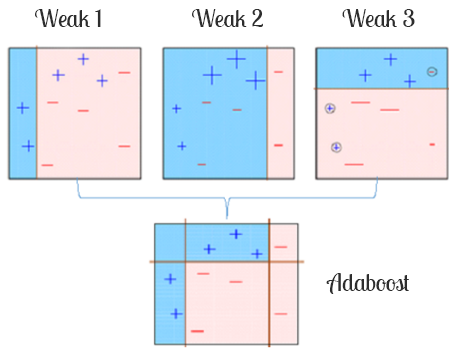
\includegraphics[width=\linewidth]{imgs/adaboost.png}
  \caption{Adaboost com 3 classificadores fracos}
  \label{fig:adaboost}
\end{figure}


